\documentclass[12pt]{report}

\usepackage[a4paper,width=150mm,top=25mm,bottom=25mm,bindingoffset=6mm]{geometry}
\usepackage[onehalfspacing]{setspace}
\usepackage{ucs}
\usepackage[table,xcdraw]{xcolor}
\definecolor{mColor1}{rgb}{0.9,0.9,0.9}

\usepackage{fancyhdr}
\pagestyle{fancy}
\fancyhead{}
\renewcommand{\chaptermark}[1]{\markboth{#1}{}}
\renewcommand\sectionmark[1]{\markright{\thesection\ #1}}

\fancyhead[LO, RE]{\leftmark}
\fancyhead[LE, RO]{\rightmark}

\usepackage{titlesec, blindtext, color}
\definecolor{gray75}{gray}{0.75}
\usepackage{mathptmx}
\usepackage[utf8]{inputenc}
\usepackage[T1]{fontenc}
\usepackage[ngerman]{babel}

\usepackage{amsmath,amssymb,amstext,amsthm,mathtools}
\usepackage{url}
\usepackage{caption}
%\usepackage[belowskip=-5pt,aboveskip=0pt]{caption}
\usepackage{subcaption}

\usepackage{float}
\usepackage{lscape}
\usepackage{pdfpages}
\usepackage{rotating}
\usepackage{graphicx}
\setlength\parindent{0pt}
\usepackage{hyperref}
\usepackage{acronym}
\usepackage{textcmds}
\usepackage{longtable}
\usepackage[export]{adjustbox}
\usepackage{upgreek}
\usepackage{dsfont}
\usepackage{tensor}
\usepackage{amsbsy}
\usepackage{multirow, hhline, colortbl}
\usepackage[table]{xcolor}


\DeclareMathAlphabet{\mathcal}{OMS}{cmsy}{m}{n}
\SetMathAlphabet{\mathcal}{bold}{OMS}{cmsy}{b}{n}

\usepackage{listings, lstautogobble}
\usepackage{textcomp}
\definecolor{yo}{rgb}{0.9,0.6,0}
\definecolor{Gray}{gray}{0.9}
\definecolor{listinggray}{gray}{0.9}
\definecolor{lbcolor}{rgb}{0.95,0.95,0.95}
\definecolor{greylines}{rgb}{0.9529,0.9529,0.9529}

\lstset{
	backgroundcolor=\color{lbcolor},
	tabsize=4,
	rulecolor=,
	language=python,
        basicstyle=\scriptsize,
        upquote=true,
        aboveskip={1.5\baselineskip},
        columns=fixed,
        showstringspaces=false,
        extendedchars=true,
        breaklines=true,
        prebreak = \raisebox{0ex}[0ex][0ex]{\ensuremath{\hookleftarrow}},
        frame=lines,
        showtabs=false,
        showspaces=false,
        showstringspaces=false,
        identifierstyle=\ttfamily,
        keywordstyle=\color[rgb]{0.55,0,0},
        alsoletter={/,*,[,]},%
        otherkeywords={},
        morekeywords=[2]{with, as},
        morekeywords=[3]{},
        emph={self},          % Custom highlighting
		emphstyle=\color[rgb]{0.1,0.3,1},
		emph={[2]f},          % Custom highlighting
		emphstyle={[2]\color[rgb]{0.1,0.5,0.1}},
		emph={[3]__init__},          % Custom highlighting
		emphstyle={[3]\color[rgb]{0.1,0.3,1}},
		emph={[4]open,str,print,KeyError},          % Custom highlighting
		emphstyle={[4]\color[rgb]{0.2,0.6,0.8}},
        commentstyle=\color[rgb]{0.3,0.3,0.3},
        stringstyle=\color[rgb]{0.133,0.545,0.133},
        	autogobble=true
}
\lstnewenvironment{ttlisting}{\lstset{basicstyle=\scriptsize}}{}

\usepackage{color}
\usepackage[section]{placeins}

\newenvironment{simplechar}{%
	\catcode`\$=12
	\catcode`\&=12
	\catcode`\#=12
	\catcode`\^=12
	\catcode`\_=12
	\catcode`\~=12
	\catcode`\%=12
	\catcode`\"=12
	\catcode`\'=12
	}{}{}

\newtheoremstyle{dotless}{}{}{\itshape}{}{\bfseries}{}{ }{}

\theoremstyle{dotless}

\newtheorem{thm}{Theorem}
\newtheorem{defn}[thm]{Definition}
\newtheorem{exmp}[thm]{Example}
\theoremstyle{definition}


\begin{document}

\begin{titlepage}
	Warum bin ich nicht einfach Staubsaugervertreter geworden?
\end{titlepage}

\tableofcontents


\chapter{Grundlagen interner Modelle im Kompositbereich}

\subsubsection{Definition eines Unternehmensmodell}
Bei einem internen Risikomodell handelt es sich um ein stochastisches Modell, das mittels stochastischer Verfahren messbare Aktiv- und Passivrisiken der betrachteten Gesellschaften abbildet. \\
Dabei sollte es über die unternehmensindividuelle Modellierung der stochastischen Geschäftsgrößen die signifikanten finanziellen Auswirkungen konsistent quantifizieren und Abhängigkeitsstrukturen zwischen alle Risikogrößen berücksichtigen.\\
Zielgrößen sind die Gesamtverteilung der Geschäftsergebnisse sowie die Berechnung des benötigten Risikokapitals in einer Marktwertsicht (Anfalljahressicht).

\subsubsection{Standardformel}
\begin{itemize}
\item Anwendung vorgegebener Stressparameter / Risikofaktoren / Szenarien pro Einzelmodul (jeweils kalibriert auf den 200-Jahresstress) ergibt Einzel-SCR
\item Jeweils Ein-Punkt-Betrachtung aller Risiken (Value-at-Risk Ansatz)
\item Anschließende Aggregation der Einzel-SCRs mit der Wurzelformel anhand von vorgegebenen Korrelationsparametern.
\end{itemize}

\subsubsection{Modellierung mit einem stochastischen Unternehmensmodell}

\begin{figure}[ht]
	\centering
	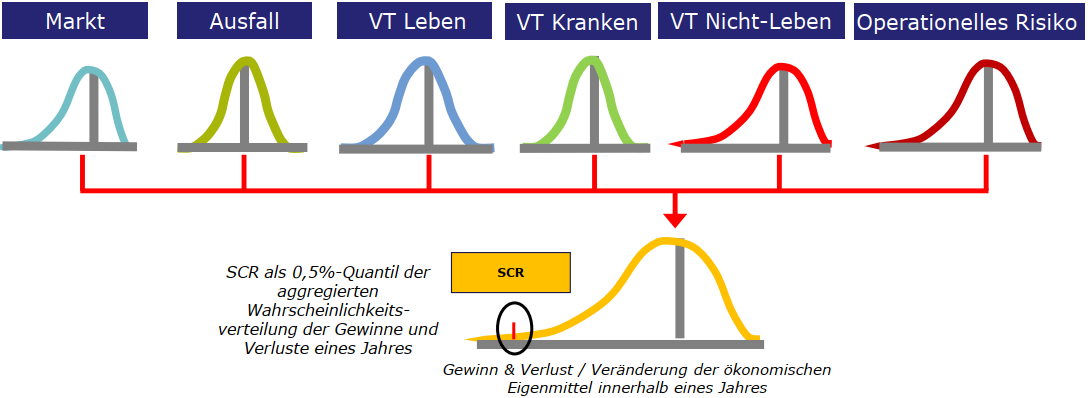
\includegraphics[width= 0.7\textwidth]{Bilder/StochUnternehmensmodell.png}
\end{figure}

\begin{itemize}
\item Simulationsbasiert: Hohe Anzahl an Simulationen erforderlich
\item separate komplette Wahrscheinlichkeitsverteilung per Risiko
\item Beliebige Risikomaße anwendbar - neben VaR auch Expected Shortfall
\end{itemize}


\subsubsection{Definitionen}
Ausgangspunkt: Gegeben seien $n \in \mathbb{N}$ Simulationswerte $(^{(1)}X, ^{(2)}X, ..., ^{(n)}X)$ einer Verlustvariable $X$ sowie das Sicherheitsniveau $\alpha \in ]0;1[$. Weiterhin bezeichne $m:= \lfloor n \cdot (1- \alpha) \rfloor$ die Gaußklammer von $n \cdot (1- \alpha)$ und $(^{(1\downarrow n)}X, ^{(2\downarrow n)}X, ..., ^{(n\downarrow n)}X)$ die obere Ordnungsstatistik mit $^{(1\downarrow n)} X \geq ^{(2\downarrow n)} X \geq ... \geq ^{(n\downarrow n)} X$

\begin{figure}[ht]
	\centering
	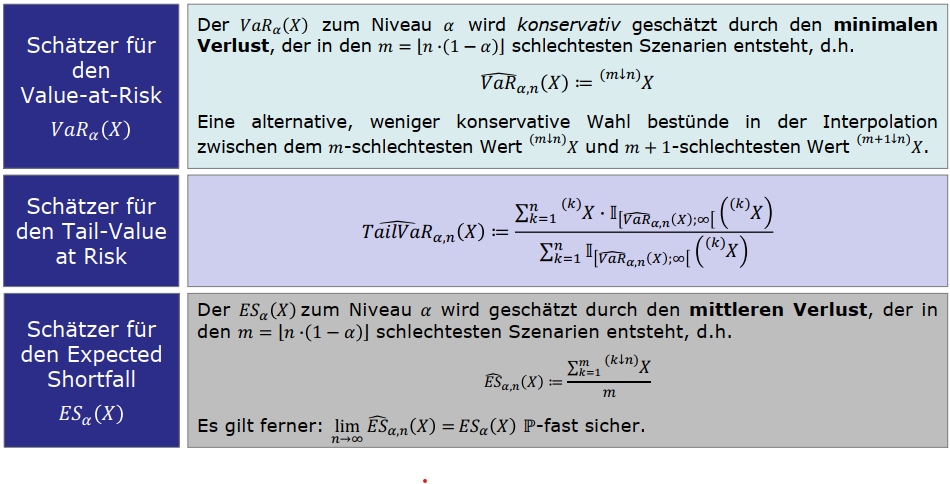
\includegraphics[width= \textwidth]{Bilder/Definitionen1.png}
\end{figure}

\subsubsection{Struktur eines DFA-Modells (Dynamische Finanzanalyse in S/U}

\begin{figure}[ht]
	\centering
	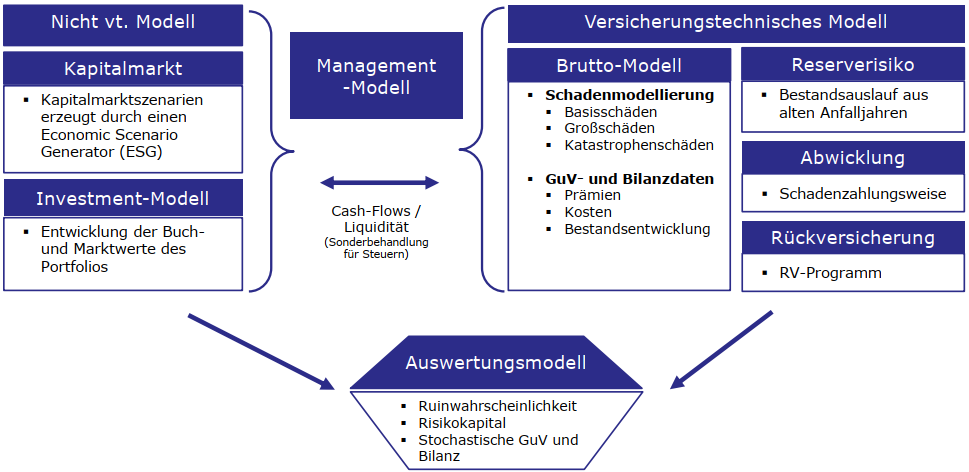
\includegraphics[width=0.8 \textwidth]{Bilder/DFA.png}
\end{figure}


\chapter{Bruttomodellierung (inkl. Katastrophenschäden)}

\section{Grundlagen}

\subsection{Zielgrößen und Gestalt der Ergebnisse}
Bei der Betrachtung des Versicherten-/ Schadenbestands lassen sich zwei Zeithorizonte bzw. Sichtweisen unterscheiden, die zu unterschiedlichen Risikodefinitionen führen:

\subsubsection{Kalenderjahressicht}

\begin{figure}[ht]
	\centering
	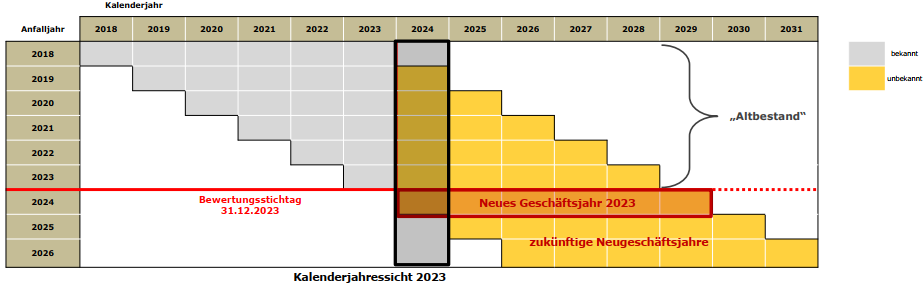
\includegraphics[width= \textwidth]{Bilder/Kalendersicht.png}
\end{figure}

\begin{itemize}
\item Neugeschäftsentwicklung im kommenden Kalenderjahr (Zahlungen + ausgehende Reserven)
\item Abwicklung des Altbestands im kommenden Kalenderjahr
\item Risikohorizont von Solvency II: Bemessungsgrundlage für die Wahrscheinlichkeit, innerhalb eines Kalenderjahres Ruin zu erleiden
\item Teilweise auch längere Zeithorizonte
\item Mögliche Verwendungszwecke: Berechnung des regulatorischen SCRs (bei internem Modell) bzw. Gesamtsolvabilitätsbedarf , Limitsysteme, Risikomarge für vt. Rückstellungen
\end{itemize}

\subsubsection{Ultimatesicht}

\begin{figure}[ht]
	\centering
	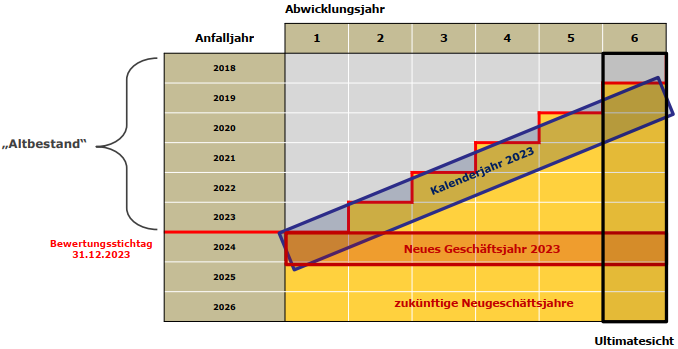
\includegraphics[width= \textwidth]{Bilder/Ultimatesicht.png}
\end{figure}

\begin{itemize}
\item Betrachtung der Ergebnisgrößen und damit verbundener Unsicherheiten über die komplette Abwicklungsdauer bis zum Endschadenstand = Ultimate auf einer Anfalljahresbasis
\item resultiert in "natürlicher" Betrachtung der vt. Risiken
\item entspricht nicht dem Risikohorizont, wie in SII für SCR vorgibt
\item Mögliche Verwendungszwecke: Profitatbilitäsmessung, Rückversicherungsanalyse, Risikozuschläge für Tarifierung
\end{itemize}

\subsection{Definition des Prämienrisikos}

Das Prämienrisiko
\begin{itemize}
\item resultiert aus der Unsicherheit / Volatilität in Bezug auf Prämien, Schaden und Kosten aus zukünftiger Risikotragung
\item bezieht sich somit nur auf diejenigen Schäden, die innerhalb des modellierten Neugeschäftsjahres (Anfalljahressicht) anfallen
\end{itemize}

Das ultimative Prämienrisiko (synonym: Zeichnungsrisiko) bezeichnet das Risiko,
dass die Prämien des Neugeschäftsjahres nicht ausreichen, um die zugehörigen Schäden
und Kosten bis zur vollständigen Abwicklung zu decken.

\subsubsection{Definition}
Das (nominale) Anfalljahresergebniss $T$ (= Technical Result) des Neugeschäftsjahres wird definiert als: $T:= P - E - U$, mit \\
P: verdiente Prämie des Neugeschäftsjahres nach vollständiger Abwicklung\\
E: Kosten des Neugeschäftsjahres nach vollständiger Abwicklung \\
U: Endschadenaufwand des Neugeschäftsjahres nach vollständiger Abwicklung \\

Das Anfalljahresergebnis $T$ ist eine Gewinnvariable: \\
$T>0$ ist äquivalent zu $P>E*U$ und bedeutet einen zukünftigen Gewinn \\
während $T<0 \Leftrightarrow P<E*U$ einen zukünftigen Verlust entspricht.

Alternative Defintion: ultimative Prämienrisiko (synonym: Zeichnungsrisiko) bezeichnet das Risiko, dass das Anfalljahresergebnis des Neugeschäftsjahres nach vollständiger Abwicklung negativ ist.

\subsubsection{Frage: Sollte man das ultimative Prämienrisiko anhand des Anfalljahresergebnisses vor oder nach Zentrierung, d.h. vor oder nach Abzug des Mittelwerts, messen?}
U.a. abhängig vom Verwendungszweck der Ergebnisse:
\begin{itemize}
\item Liegt Fokus auf Auswirkungen auf die Kapitalsituation?
\item Sind Erträge und Verluste aus zukünftigen Neugeschäft in Eigenmitteln enthalten?
\item Primär Darstellung Ergebnisvolatilität?
\item Weitere Überlegungen:
\begin{itemize}
\item Das erwartete Ergebnis (= Mittelwert der Simulationen) entspricht nicht zwingend dem geplantem Ergebnis
\item Bei hochprofitablem Geschäft ist ohne Zentrierung des originären Anfalljahresergebnisses bei bestimmten Risikomaßen (Bsp: VaR) sogar ein negatives Risikokapital möglich.
\end{itemize}
\end{itemize}

Ergebnisgrößen für das Prämienrisiko:
\begin{itemize}
\item Ergebniskomponenten:
\begin{itemize}
\item Verdiente Prämie: i.d.R. fix, bei mehrjähriger Projektion sit Prämienzyklus zu berücksichtigen
\item Kosten: getrennt nach Vertrieb, Regulierung und Verwaltung
\item Schäden: stochastische Modellierung, zwecks genauer Abbildung der Rückversicherungsstruktur und Modellierung der spartenspezifischen Schadenvolatilitätn erfolgt Trennung nach Schadentp (Einzelne Großschäden, Einzelne Ereignisse)
\end{itemize}
\item Segmentierung/ Modellierungstiefe: 
\begin{itemize}
\item Aufteilung in HUK und Sach
\item Bsp. HUK: Kasko, Haftpflicht, Unfal
\item Bsp. Sach: VGV, Feuerindustrie
\end{itemize}
\end{itemize}

\subsection{Schadenmodellierung}
Trennung der Schadentypen: Basisschäden, Großschäden, Katastrophenschäden

\subsubsection{Basisschäden}
\begin{itemize}
\item hohe Schadenfrequenz und geringe Schadenhöhe
\item Simulation als Aggregat
\item Parametrisierung auf Basis eigener Schadenerfahrung
\end{itemize}

\subsubsection{Großschäden}
\begin{itemize}
\item Schäden oberhalb spezifischen Schwellenwerts
\item geringe Frequenz, große Schadenhöhe
\item Modellierung: Einzelbasis nach dem kollektiven Modell
\item Parametrisierung auf Basis eigener Schadenerfahrung
\end{itemize}

\subsubsection{Katastrophenschäden}
\begin{itemize}
\item sehr niedrige Eintrittswahrscheinlichkeit, extreme Schadenhöhe
\item Trennung nach Naturgefahren, Man-Made Gefahren, sonstiges wie Pandemien
\item Charakteristika Naturgefahren: Treffen größere Region, Ereignisschaden setzt sich aus vielen kleinen Einzelschäden zusammen, Schäden betreffen viele Sparten gleichzeitig (Wohngebäude, Hausrat, Kraftfahrt...)
\item Charakteristika Man-Made Gefahren: hohes Schadenpotenzial neben Kumulereignisen auch einzelne Spitzenrisiken (Bsp. Fabrikgebäude)
\item i.d.R. Rückversicherungsschutz
\item Modellierung i.A. auf Basis von Einzelereignissen
\end{itemize}

\subsection{Schadenmodellierung (excl. CAT)}

\begin{figure}[ht]
	\centering
	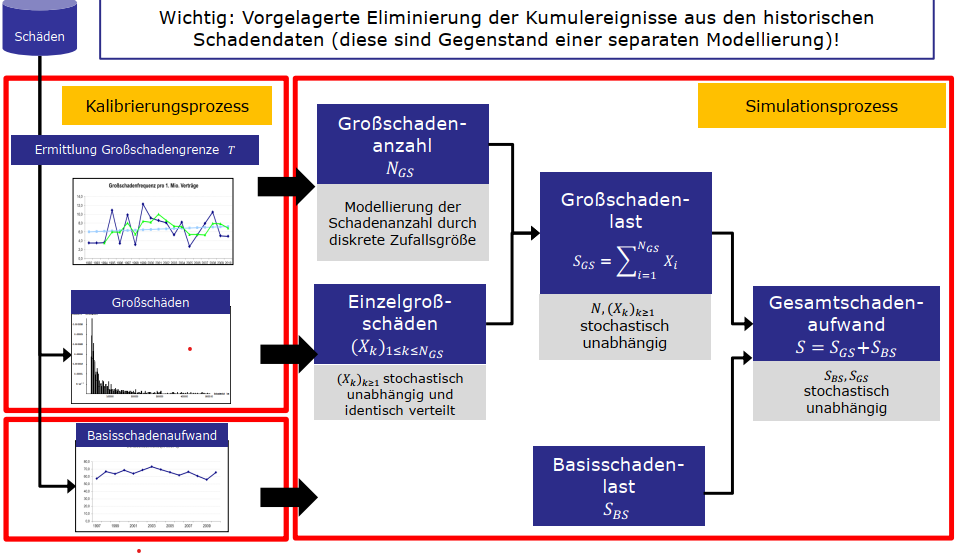
\includegraphics[width= \textwidth]{Bilder/Folie27.png}
\end{figure}

\subsubsection{Kalibrierungsprozess}
\begin{itemize}
\item Abwicklung der Schäaden (Ermittlung voraussichtlicher Endschadenstände)
\item "as if"-Transformation der Schäden (wenn der Schaden im parametrisierenden Schadenjahr angefallen wäre)
\begin{itemize}
\item Anpassung an aktuelle Bestandsgröße
\item Anpassung an momentanen Geldwert
\item Bereinigung um Trends
\end{itemize}
\item Großschadenfrequenz: Schätze Erwartungswert und Varianz für Frequenz, Anpassung Schadenzahlverteilung (Poisson, Negativ Binomial)
\item Einzelgroßschadenhöhe: Schadenhöhen Anpassung mit schwerer Verteilung: QQ-Plot, Statistische Bewertung
\item Basisschadenlast: Analyse des Schadenbedarfs
\end{itemize}


\section{Modellierung von Katastrophenschäden}

\subsubsection{Definition}
Laut Solvency II stellt das Katastrophenrisiko das Risiko eines außergewöhnlich großen Ereignisses dar – gemäß Rahmenrichtlinie Artikel 105 (2) bezeichnet das Katastrophenrisiko Nicht-Leben das „Risiko eines Verlustes oder einer nachteiligen Veränderung des Werts der Versicherungsverbindlichkeiten, das sich aus einer signifikanten Ungewissheit in Bezug auf die Preisfestlegung und die Annahmen bei der Rückstellungsbildung für extreme oder außergewöhnliche Ereignisse ergibt“.

Beispiel Naturgefahren: Überschwemmung, Hagel, Erdbeben, ... \\
Beispiel Man-Made Gefahren: Explosion, Terror, Cyberangriffe, Luftfahrtunglück

\subsubsection{Analyse und Bewertung des Katastrophenpotentials der versicherten Gefahren}

\begin{itemize}
\item Analyse der Bruttoexponierung (Versicherungssumme, Prämienvolumen,…),
\item Umfang an Rückversicherungsschutz
\item Historische Schäden des Unternehmens, Referenzschäden aus dem Markt
\item Ergebnisse von Quantifizierungsansätzen – Beispiele:
\item Solvency II-Standardformel
\item Externe Modelle
\item Mathematisch-statistische Modellierung
\item Szenarioanalysen
\item Externe (Markt-)einschätzung / Externe Analysen
\item Ergebnis: Qualitative / Quantitative Einschätzung der Materialität jeder Gefahr, Gegenüberstellung mit geeigneter Bezugsgröße des Unternehmens (wie Solvenzkapitalbedarf, Eigenmittel)
\end{itemize}


\subsubsection{Analyse und Bewertung der Datenverfügbarkeit /-qualität}

\begin{itemize}
\item Exposuredaten (Informationen in der benötigten Detailtiefe für den Bestand vorhanden?)
\item Historische Schadendaten
\end{itemize}

\subsection{Charakterisierung von Katastrophenschadenverteilungen}

\begin{itemize}
\item Erwartungswert und Standardabweichung wenig aussagekräftig
\item Daraus folgt: Komplette Verteilungsfunktion benötigt
\item Zwecks Darstellung und Vergleich von Katastrophenschadenverteilungen (auf Jahresbasis) bietet sich die Übersetzung in sog. Überschreitungswahrscheinlichkeiten / Wiederkehrperioden an:
\begin{itemize}
\item Schadenhöhe, die nur in $x\%$ aller Jahre überschritten wird: Ereignis weist eine jährliche Überschreitungswahrscheinlichkeit von $x\%$ auf.
\item Schadenhöhe, die im Mittel nur alle $T$ Jahre beobachtet wird: Ereignis weist die Wiederkehrperiode / Jährlichkeit $T$ auf.
\end{itemize}
\end{itemize}

\subsubsection{Definition}
Bezeichne $N$ die zufällige Anzahl an Ereigniseintritten in einem Jahr und $X_1, ..., X_N$ die zugehörigen Ereignisschadenhöhen sowie\\
$M_N:= max{\{ X_1, ..., X_N\}}$ den max. Ereignisschaden eines Jahres (mit $M_N=0$ für $N=0$)\\
$S:= \sum^N_{i=1} X_i$ den Jahresgesamtschaden \\
Seien weiter $F_{M_N}$ die Verteilungsfunktion von $M_N$ sowie $F_S$ die Verteilungsfunktion von $S$ und $F^{-1}_{M_N}$ und $F^{-1}_S$ihre zugehörigen Inversen. \\
Dann ergeben sind OEP-Kurve und AEP-Kurve als Punktepaare $(T, OEP(T))$ bzw. $(T, AEP(T))$ mit $T \in [1;\infty ]$ und
\begin{equation}
OEP(T) := F^{-1}_{M_N} \left( 1- \frac{1}{T} \right) , AEP(T):= F^{-1}_S \left( 1- \frac{1}{T} \right)
\end{equation}
Die OEP-Kurve stellt den maximalen Ereignisschaden eines Jahres (Maximum Occurrence Loss) in
Abhängigkeit der Wiederkehrperiode dar, die AEP-Kurve wiederum den Jahresgesamtschaden (Annual
Aggregate Loss) \\

Liegen simulierte Ereignisse aus dem Simulationsmodell vor, lassen sich die AEP und OEP-Kurven
aus den empirischen Verteilungen des maximalen jährlichen Ereignisschadens und
Jahresgesamtschadens bestimmen. 

\begin{figure}[ht]
	\centering
	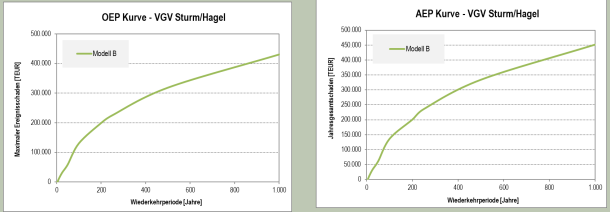
\includegraphics[width= \textwidth]{Bilder/OEPAEP.png}
\end{figure}
 \vspace{4cm}
Für OEP-Kruve ist unter bestimmten Voraussetzung auch analytische Ermittlung möglich:
\begin{figure}[ht]
	\centering
	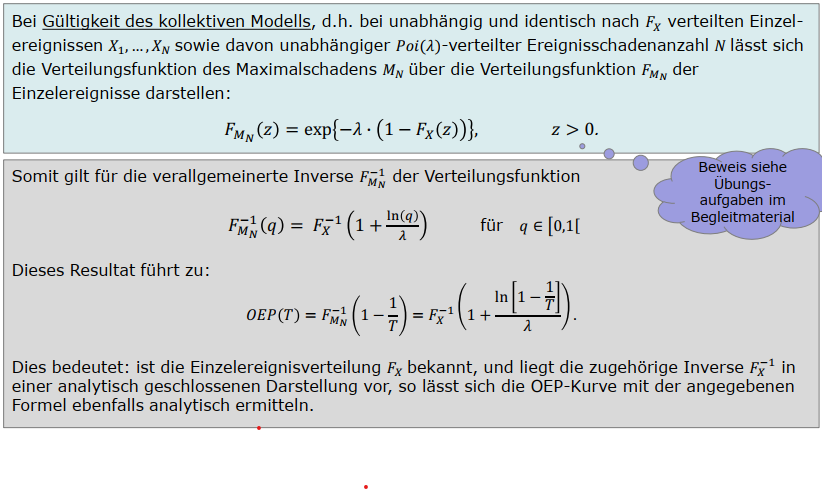
\includegraphics[width= \textwidth]{Bilder/Folie39.png}
\end{figure}

\subsection{Modellierungsansätze für Katastrophenschäden}

\begin{itemize}
\item Mathematisch-statistische Modelle: \\
Schaden wird basierend auf der Schadenerfahrung mit klassischen aktuariellen Verfahren
\item Exposure-basierte probabilitische Modelle: \\
zunächst die schadenbestimmende Ursache eines Ereignisses simulieren und anschließend ihre Schadenwirkungen auf die versicherten Risiken des Unternehmens (Exposure) bestimmt. (Naturgefahrenbereich: geophysikalisch-meteorologische Modelle)
\item Szenario-basierte Modelle: \\
Schadenpotential wird anhand von Szenarioanalysen geschätzt. Schadenhöhe und Eintrittswahrscheinlichkeit bzw. Wiederkehrperiode eines oder mehrerer Einzelszenarien werden mit Hilfe von Verteilungsannahmen in eine Wahrscheinlichkeitsverteilung übersetzt.
\end{itemize}


\subsubsection{mathematisch-statistische (aktuarielle) Modellierung}
Unterteilung in:
\begin{itemize}
\item Explizite Modellierung: im Modell liegt eine eigenständige Katastrophenschadenverteilung für diese Gefahr vor.
\item Implizite Modellierung: keine eigene Katastrophenschadenverteilung, stattdessen: 
\begin{itemize}
\item Die Gefahr wird entweder gemeinsam mit anderen Gefahren modelliert
\item Katastrophenschäden dieser Gefahr werden gemeinsam mit anderen Schadenarten (Basis- oder Großschäden) modelliert
\item Loading: Zuschlag auf Gesamtebene
\end{itemize}
\end{itemize}


\subsection{Explizite Modellierung gemäß mathematisch-statistischer Ansätze}

\subsubsection{Allgemeine Methodik/ Vorgehen}
\begin{itemize}
\item Katastrophenschadenverteilung ergibt sich aus der Anpassung geeigneter Wahrscheinlichkeitsverteilungen an Ereignisschadenhöhen und –anzahlen oder direkt an Jahresschadenlast
\item aus Basis historischer Schadendaten (unternehmenseigene Schadenhistorie) nach as-if Transformation
\end{itemize}

\subsubsection{Mögliche Ansätze/ Beispiele}
\begin{itemize}
\item Ereignisschadenhöhe bedarf in der Regel hinreichend schwerer Verteilung (Bsp: Pareto)
\item Ggf. auch differenziertere, zweistufige Modellierung der Ereignisschadenhöhe
\item Sofern verfügbar: Einbezug von Marktschadendaten
\end{itemize}


\subsection{Implizite Modellierung gemäß mathematisch-statistischer Ansätze}

Folie 46
































\end{document}